% +------------------------------------------------------------------------+
% | Reference manual page: Subdivision_surfaces_3.tex
% +------------------------------------------------------------------------+
% | 03/01/2005   Le-Jeng Andy Shiue
% | Package: Subdivision_surface_3
% | 
\RCSdef{\RCSSubdivisionRev}{$Revision$}
\RCSdefDate{\RCSSubdivisionDate}{$Date$}
% +------------------------------------------------------------------------+

\ccRefPageBegin

%%RefPage: end of header, begin of main body
% +------------------------------------------------------------------------+


\begin{ccRefClass}{Subdivision_surfaces_3}

\ccDefinition

Subdivision surfaces of an input polyhedral mesh (i.e.~control mesh)
are generated by recusive connectivity refinement and geometry
smoothing. \ccClassTemplateName\ consists a set of static 
template functions (i.e.~refinement hosts) corresponding 
to four refinement schemes practically by used subdivision algorithms. 
Each refinement host, parameterized with a policy class
consisting of a set of geometry stencils, refines the
control mesh and assigns smoothed nodes on the refined mesh
by excuting geometry averaging provided by the policy class.
Another set of subdivision functions are also provided  
for Catmall-Clark, Loop, Doo-Sabin and $\sqrt{3}$ subdivision.
These subdivision functions are pre-parameterized with the
subdivision geometry stencils.

%% \begin{ccTexOnly}
%%     \vspace{-7mm}
%%     \begin{center}
%%       \parbox{0.4\textwidth}{%
%%         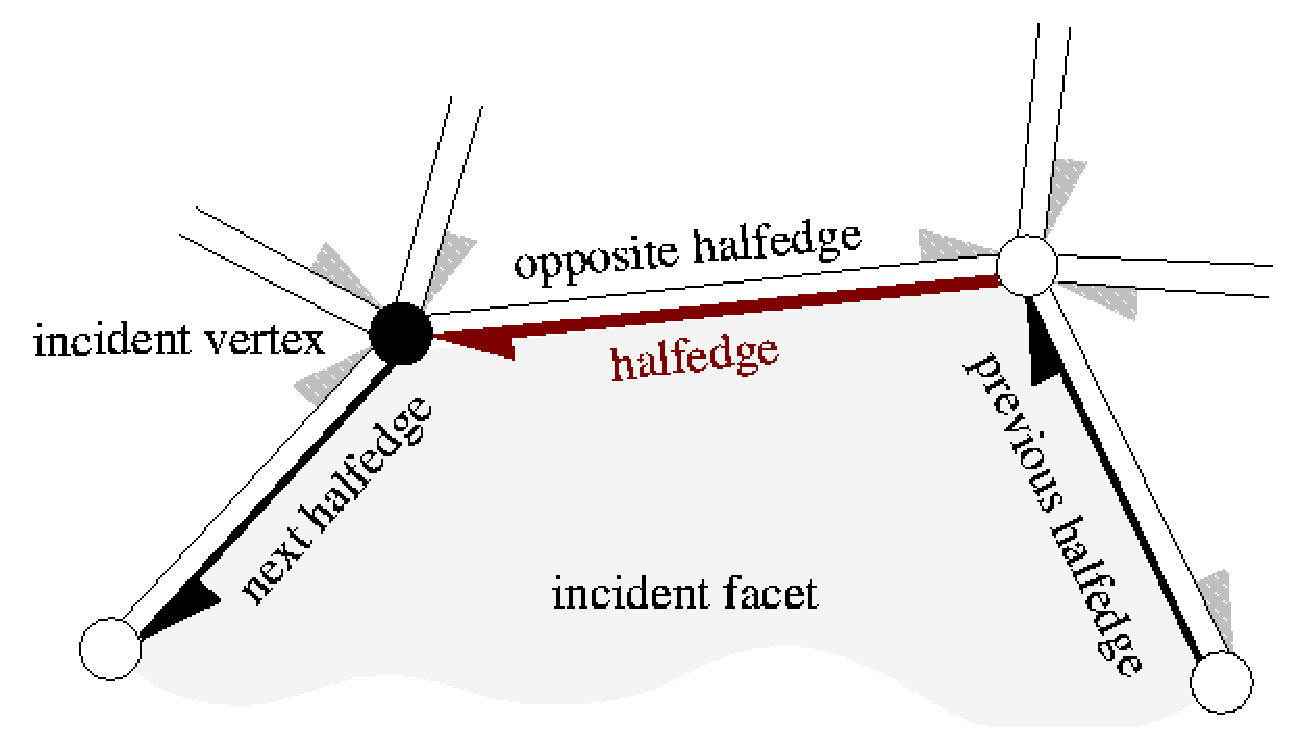
\includegraphics[width=0.4\textwidth]{Polyhedron_ref/fig/halfedge}%
%%       }
%%     \end{center}
%%     \vspace{-5mm}
%% \end{ccTexOnly}

%% \begin{ccHtmlOnly}
%%     <CENTER>
%%     <A HREF="fig/halfedge.gif">
%%         <img src="fig/halfedge_small.gif" alt="Halfedge Diagram"></A><P>
%%     </CENTER>
%% \end{ccHtmlOnly}

\ccInclude{CGAL/Subdivision_surfaces_3.h}

\ccParameters

The full template declaration of \ccClassTemplateName\ states one
template parameters:

\begin{tabbing}
\ccc{template <} \=\ccc{class  _Poly>}\\
     \ccc{class Subdivision_surfaces_3;}
\end{tabbing}
   
The \ccc{_Poly} parameter requires a model of 
the \ccc{Polyhedron_3} concept as argument. The storage structure
of the \ccc{_Poly} (e.g.~list or vector) is required to be
FIFO sturucture, since the iteration order of vertices is used
to encode the stencils defined between the input mesh and the refined
mesh. \ccc{Point_3} type is reqiured to be defined in the \ccc{_Poly}.

%% \ccTypes

%% \ccNestedType{Traits}{traits class selected for \ccc{PolyhedronTraits_3}.}
%% \ccGlue
%% \ccNestedType{Items}{items class selected for \ccc{PolyhedronItems_3}.}
%% \ccGlue



%% % +-----------------------------------+
%% \begin{ccAdvanced}
%% \ccHeading{Types for Tagging Optional Features}

%% \ccNestedType{Supports_facet_plane}{\ccc{Facet::plane()}.}
%% \ccGlue
%% \ccNestedType{Supports_removal}{supports removal of individual elements.}

%% \end{ccAdvanced}

\ccCreation
%\ccCreationVariable{P}

\ccClassTemplateName\ serves as namespcae arameterized with
the \ccc{_Poly}, and provides a set of static refinement 
functions. 
%No object of \ccClassTemplateName\ is reuqired to be 
%instantiated before calling subdivision or generic refinement functions.

% +-----------------------------------+
\ccHeading{Refinement hosts}

\ccThree{}{}{}
\ccMethod{template <template <typename> class _S> 
void PQQ(Polyhedron& p, _S<Polyhedron> rule, int step)}
{refine the mesh \ccc{p} with the PQQ scheme 
\ccc{step} times, and assign the smoothed points with the geometry 
stencils \ccc{rule}.}
%% \begin{ccTexOnly}
%%     \begin{center}
%%       \parbox{0.636\textwidth}{%
%%           \includegraphics[width=0.636\textwidth]%
%%               {Polyhedron_ref/fig/euler_loop}%
%%       }
%%     \end{center}
%% \end{ccTexOnly}
%% \begin{ccHtmlOnly}
%%     <CENTER>
%%     <img src="fig/euler_loop.gif" alt="Euler Operator: Loop"><P>
%%     </CENTER>
%% \end{ccHtmlOnly}

\ccMethod{template <template <typename> class _S> 
void PTQ(Polyhedron& p, _S<Polyhedron> rule, int step)}
{refine the mesh \ccc{p} with the PTQ scheme 
\ccc{step} times, and assign the smoothed points with the geometry 
stencils \ccc{rule}.}

\ccMethod{template <template <typename> class _S> 
void DQQ(Polyhedron& p, _S<Polyhedron> rule, int step)}
{refine the mesh \ccc{p} with the DQQ scheme 
\ccc{step} times, and assign the smoothed points with the geometry 
stencils \ccc{rule}.}

\ccMethod{template <template <typename> class _S> 
void Sqrt3(Polyhedron& p, _S<Polyhedron> rule, int step)}
{refine the mesh \ccc{p} with the Sqrt(3) scheme 
\ccc{step} times, and assign the smoothed points with the geometry 
stencils \ccc{rule}.}


% +-----------------------------------+
\ccHeading{Subdivision Algorithms}
\ccThree{}{}{}

\ccMethod{void CatmullClark_subdivision(Polyhedron& p, int step)}
{apply Catmull-Clark subdivision on the mesh \ccc{p} \ccc{step} times.}

\ccMethod{void Loop_subdivision(Polyhedron& p, int step)}
{apply Loop subdivision on the mesh \ccc{p} \ccc{step} times. 
The mesh \ccc{p} can only consist of triangle factes.}

\ccMethod{void DooSabin_subdivision(Polyhedron& p, int step)}
{apply Doo-Sabin subdivision on the mesh \ccc{p} \ccc{step} times.}

\ccMethod{void Sqrt3_subdivision(Polyhedron& p, int step)}
{apply Sqrt(3) subdivision on the mesh \ccc{p} \ccc{step} times.
The mesh \ccc{p} can only consist of triangle factes.}

\ccSeeAlso

\ccRefIdfierPage{CGAL::Subdivision_surfaces_rules_3}

\ccExample

This example program applies the Catmull-Clark subdivision on the
read-in polyhedral mesh.

\ccIncludeExampleCode{Subdivision_surfaces_3/CatmullClark_subdivision.C}

\end{ccRefClass}

% +------------------------------------------------------------------------+
%%RefPage: end of main body, begin of footer
\ccRefPageEnd
% EOF
% +------------------------------------------------------------------------+
